\documentclass[a4paper,11pt]{article}

\usepackage{bm,amsmath,amsfonts,amsthm}
\usepackage{mathpazo,microtype,setspace,parskip}
\usepackage[margin=2cm, bottom=2.5cm]{geometry}
\usepackage{float}
\usepackage{booktabs}
\usepackage{graphicx}
\usepackage{natbib}
\usepackage[no-weekday]{eukdate}
\usepackage[margin=.5cm]{caption}
\captionsetup[figure]{font=footnotesize,labelfont=footnotesize}
\captionsetup[table]{font=footnotesize,labelfont=footnotesize}
\usepackage{color}
\usepackage[colorlinks,linkcolor=black,citecolor=black,filecolor=black,bookmarks=false]{hyperref}
\usepackage[capitalize,nameinlink]{cleveref}

\newcommand{\dt}{\mathrm{d}}
\newcommand{\E}{\mathbb{E}}

\newtheorem{assumption}{Assumption}
\newtheorem{theorem}{Theorem}
\newtheorem{corollary}{Corollary}
\newtheorem{lemma}{Lemma}
\newtheorem{example}{Example}

\setstretch{1.3}

\begin{document}
\title{Anomaly detection using surprisals}
\author{Rob J Hyndman and David T Frazier}

\maketitle

\begin{abstract}
	TBC
\end{abstract}

\noindent\textbf{Keywords:}
Extreme value theory;
Generalized Pareto Distribution;
Outlier detection;
Tail bounds.

\section{Introduction}

Let $y_1,\dots,y_n$ be observations from a probability distribution $F$. The \emph{surprisal} of observation $y_i$ is defined as \citep{Stone2022}
$$
	s_i=-\log f(y_i),
$$
where $f$ is either the density or probability mass function of $F$. While these are better known as ``log scores'' in statistics \citep{Good1952-zw}, in this context we prefer the term ``surprisal'' \citep[coined by][]{Tribus61},  as it captures the idea that observations with low density are more ``surprising'' (and therefore potentially anomalous) than those with high density.

Let $G(s) = P(S\le s)$ be the distribution function of the surprisal values,  where $S = -\log f(Y)$ and $Y\sim F$. Then, the probability of observing a value with surprisal at least as large as $s$ is given by $1-G(s)$, which leads to a natural way to assign an anomaly score to each observation $y_i$:
$$
	p_i = 1-G(s_i) = 1-G(-\log f(y_i)).
$$
Hence, one way to detect anomalies is to flag observations with $p_i < \alpha$, giving a false positive rate of $\alpha$. This is preferable to directly computing the probabilities from the tail of $F$, as it allows for anomalies to occur anywhere in the distribution of $F$, not just in its tails. For example, anomalies may lie between modes in a multimodal distribution, or in otherwise low-density regions of the distribution $F$.

However, we will usually not know $F$, and so we need to estimate it from data or from theory. Such estimates are particularly fragile in areas of low density, which is precisely where we are looking for anomalies.

To address this, \citet{lookout} proposed estimating $F$ by a leave-one-out kernel density estimate, and then fitting a Generalized Pareto Distribution (GPD) to the most extreme surprisal values. \citet{lookout2} provides some theoretical justification for this approach. The underlying idea is that even if $F$ is not particularly well-estimated, the tail of the surprisal distribution should still be well-approximated by a GPD.

Here we extend that idea to allow $F$ to be any well-behaved distribution, including conditional distributions. Specifically, we fit a GPD to the largest $\beta$ of $\{-\log f_i\}_{i=1}^n$, obtaining estimates of the location, scale and shape parameters, $(\mu,\sigma,\xi)$. We calculate the probability of each observation or one more extreme, $p_i = \beta\left[1-P(-\log f_i \mid \hat\mu, \hat\sigma, \hat\xi)\right]$, where $P$ is the distribution function of the GPD. Observations not contained in the largest $\beta$ of $\{-\log f_i\}_{i=1}^n$ are assigned $p_i = \beta$.

To justify this approach, we seek conditions on the surprisal distribution of $S = -\log f(Y)$, where $Y\sim F$, similar to the Fisher-Tippett-Gnedenko (FTG) theorem \citep{coles2001introduction}.

\section{Assumptions and preliminary results}

Before establishing the main results, we need to place some assumptions on the data generating process.

\begin{assumption}\label{ass:iid}
	The sequence $y_i$ is iid from $F$.
\end{assumption}

Under \cref{ass:iid}, we have that $s_i=-\log f(y_i)$ is also iid, and its distribution function is given by
$$
	G(s) = \mathrm{Pr}(S\le s) = \mathrm{Pr}\{-\log f(Y)\le s\} = \Pr\{ f(Y)\ge e^{-s}\}.
$$
This makes clear that the surprisal probability is related to the highest density regions of the distribution \citep{HDR96}. In fact, every observation with $p_i< \alpha$ lies outside the $100(1-\alpha)$\% HDR region of $F$.

Next we need to place some conditions on the surprisal distribution. We consider three possibilities describing increasingly heavy tails: (1) where $S$ is sub-Gaussian (which occurs when $f$ is bounded above and below); (2) where $S$ is sub-exponential; and (3) where $S$ has a polynomial moment. We state these as three alternative assumptions.

\begin{assumption}[Sub-Gaussian]\label{ass:bounded}
	The random variable $S =-\log f(Y)\in\mathbb{R}$, and satisfies, for all $\lambda\in\mathbb{R}$, and some $\nu>0$,
	$$
		\E \exp\{\lambda (S-\E[S])\}\le \exp\{\lambda^2 \nu^2/2\}.
	$$
\end{assumption}

\begin{assumption}[Sub-exponential]\label{ass:subbounded}The random variable $S$ is sub-exponential with parameters $\nu$ and $b$, i.e.,
	$$
		\E \exp\{\lambda(S-\E[S])\} \leq \exp\{\lambda^2\nu^2/ 2\} \quad\text{ for all } \quad |\lambda|< 1/b.
	$$
\end{assumption}

\begin{assumption}[Polynomial]\label{ass:polybounded}
	The random variable $|S|$ has polynomial moments of order $\alpha\ge 1$; i.e.,
	$\mathbb{E}[|S|^p] \le C^p$ for some $C>0$ such that $C^p-1>0$.
\end{assumption}

Under \cref{ass:iid}, and one of Assumptions \ref{ass:bounded}--\ref{ass:polybounded}, we seek a result on the limiting distribution of the maximum of the surprisals $M_n = \max\{s_1,\dots,s_n\}$. If we can show that this distribution falls within the class of extreme value distributions, then we can fit a Generalized Pareto Distribution to the largest surprisal values \citep{coles2001introduction}.

\subsection{$S$ has sub-Gaussian tails}

Let's first assume that the surprisals are well-behaved and have a sub-Gaussian tail. \cref{ass:bounded} will be satisfied in cases where the density $f$ is bounded both above and below, such as with mass functions on a finite set. However, it may not be satisfied if the density has no lower bound.

For example, consider the truncated normal distribution on $[a,b]$, where $Y\sim \mathcal{TN}(a,b,\mu,\sigma^2)$ and $-\infty < a < b < \infty$. Then
$$
	S=-\log(2\pi\sigma^2)/2-\frac{1}{2\sigma^2}(Y-\mu)^2-\log\{\Phi(b)-\Phi(a)\},
$$
where $\Phi$ is the standard normal distribution function. Since $Y\in[a,b]$, $S$ is bounded for all $\sigma>0$ and hence $S$ satisfies \cref{ass:bounded}.

Under Assumptions \ref{ass:iid} and \ref{ass:bounded}, we have the following result on the maximum of the surprisals $M_n = \max\{s_1,\dots,s_n\}$.
\begin{lemma}\label{lem:bounds}
	If Assumptions \ref{ass:iid}--\ref{ass:bounded} are satisfied, then, for $s\in\mathbb{R}_+$,
	$$
		\mathrm{Pr}(M_n-\E[S]\ge s)\le 1-\left\{1-e^{-\frac{1}{2}s^2/\nu^2}\right\}^n.
	$$
\end{lemma}

\begin{proof}
	For any $\lambda>0$,
	\begin{align*}
		\Pr\{S\ge s\} =
		\Pr\left\{e^{\lambda (S-\E[S])}\ge e^{\lambda (s-\E[S])}\right\}
		 & \le e^{-\lambda(s-\mu)}\E e^{\lambda (S-\mu)}  \\
		 & \le  e^{-\lambda(s-\mu)}e^{\lambda^2\nu^2/2} .
	\end{align*}
	Now, we can maximise the RHS of the above bound in $\lambda$, which yields the optimal value $\lambda=(s-\mu)/\{M^2\}$. Plugging this in we have the bound
	$$
		\Pr\{S\ge s\}\le e^{-\frac{1}{2}(s-\mu)^2/\nu^2}.
	$$
	The stated result now follows by noting that
	\begin{align*}
		\mathrm{Pr}\left(M_n-\E[S]\ge s\right) = 1-\mathrm{Pr}\{M_n\le s\}
		 & = 1-\mathrm{Pr}\{S\le s\}^n            \\
		 & = 1-(1-\Pr\{S\ge s\})^n                \\
		 & \le 1-(1-e^{-\frac{1}{2}s^2/\nu^2})^n.
	\end{align*}
\end{proof}
\begin{corollary}\label{cor:one}
	If Assumptions \ref{ass:iid}--\ref{ass:bounded} are satisfied, then, for all $s>0$,
	$$
		\mathrm{Pr}\Big(|M_n-\E[S]| \ge \sqrt{2\nu^2s} + \sqrt{2\nu^2\log(2n)}\Big) \le e^{-s}.
	$$
\end{corollary}
\begin{proof}
	This follows directly from the union bound:
	\begin{align*}
		\mathrm{Pr}\Big(|M_n|\ge \sqrt{2\nu^2s} + \sqrt{2\nu^2\log(n)}\Big)
		 & \le n \Pr\Big\{|S|\ge \sqrt{2}\nu^2s + \sqrt{2\nu^2\log(n)}\Big\}                                                     \\
		 & \le 2n e^{-[\sqrt{2\nu^2s}+\sqrt{2\nu^2\log(n)}]^2/(2\nu^2)}                                                          \\
		 & = 2n e^{-\frac{1}{2\nu^2}(2s\nu^2 )-\frac{2\nu^2\log(2n)}{2\nu^2}-\frac{\sqrt{2\nu^2s}\sqrt{2\nu^2\log(2n)}}{2\nu^2}} \\
		 & \le e^{-\sqrt{\log(2n)s}-s}                                                                                           \\
		 & \le e^{-s}
	\end{align*}
	The first result follows from the iid assumption on $S$ and the union bound, while the second from the assumption that $S$ is sub-Gaussian. The remaining inequalities follow from reorganising terms.
\end{proof}

\cref{cor:one} is useful as it clarifies that if the surprisal is sub-Gaussian, then the maximal surprisal will follow a reversed Weibull distribution, and thus is within the class of extreme value distributions.

\subsection{$S$ has an exponential moment}

In cases where the underlying density has full support on $\mathbb{R}$ and cannot be bounded from below, then the sub-Gaussianity condition in \cref{ass:bounded} may be violated, as the following result illustrates.

\begin{lemma}
	If $Y\sim \mathcal{N}(\mu,\sigma^2)$, then $S=-\log f(Y)$ is sub-exponential. In particular,
	$$
		\E e^{\lambda(S-1/2)+(\lambda/2)\log(2\pi\sigma^2)}\le e^{\lambda^2/2+(\lambda/2)\log(2\pi\sigma^2)},\quad \forall |\lambda|<1/2.
	$$
\end{lemma}
\begin{proof}
	Firstly, note that
	$$
		S=-\log f(Y)= \frac{1}{2}\log (2\pi\sigma^2)+\frac{(Y-\mu)^2}{2\sigma^2}.
	$$
	and that
	$$
		\mu_S=\E[S]=-\int f(y)\log f(y)\dt y=\frac{1}{2}\{1+\log (2\pi\sigma^2)\}.
	$$ Define
	$$
		X=\frac{1}{2}\frac{(Y-\mu)^2}{\sigma^2}-\frac{1}{2},
	$$
	then $\E[X]=0$. Now, note that
	$$
		\E e^{\frac{\lambda}{2}(S-1)}={e^{\lambda/2\{\log(2\pi\sigma^2)\}}}\frac{1}{\sqrt{2\pi\sigma^2}  }\int e^{\frac{\lambda}{2}\left[\frac{(y-\mu)^2}{\sigma^2}-1\right]}e^{-\frac{(y-\mu)^2}{2\sigma^2}}\dt y.
	$$
	Consider the change of variables $z=(y-\mu)/\sigma$ so that we have
	$$
		\E e^{\frac{\lambda}{2}(S-1)}={e^{\lambda/2\{\log(2\pi\sigma^2)\}}}\frac{1}{\sqrt{2\pi}  }\int e^{\frac{\lambda}{2}[z^2-1]}e^{-z^2/2}\dt y={e^{\lambda/2\{\log(2\pi\sigma^2)\}}}\frac{e^{-2(\lambda/2)}}{\sqrt{1-2(\lambda/2)}}
	$$for all $\lambda<1$. Further, it can be verified that
	$$
		\frac{e^{-\lambda/2}}{\sqrt{1-2(\lambda/2)}}\le e^{\lambda^2/2},\quad \forall |\lambda|<1/2.
	$$
	Hence, when we have $Y\sim\mathcal{N}(\mu,\sigma^2)$, then $S=-\log f(Y)$ is sub-exponential with parameter $\nu=1$ and $b=2$.
\end{proof}

Therefore, to be able to apply extreme value theory to the surprisal values, we need a version of \cref{lem:bounds} that uses sub-exponentiality.


\begin{lemma}\label{lem:bounds_sub}
	If Assumptions \ref{ass:iid} and \ref{ass:subbounded} are satisfied, then, for $s\in\mathbb{R}_+$,
	$$
		\mathrm{Pr}\left(M_n-\E[S]\ge s\right)\le 1-
		\begin{cases}
			(1-e^{-\frac{1}{2}s^2/\nu^2})^n & \text{ if }0\le s\le \nu^2/b \\
			(1-e^{-s/2b})^n                 & \text{ if }s>\nu^2/b
		\end{cases}.
	$$
\end{lemma}
\begin{proof}
	The result follows a similar argument as for \cref{lem:bounds}, up until we maximize the tail bound. In particular, for any $\lambda>0$,
	\begin{align*}
		\Pr\left\{ S-\E[S]\ge s\right\} =
		\Pr\left\{e^{\lambda (S-\E[S])}\ge e^{\lambda s}\right\}
		 & \le e^{-\lambda s}\E e^{\lambda (S-\E[S])} \\
		 & \le  e^{-\lambda s}e^{\lambda^2\nu^2/2} .
	\end{align*}
	Now, we must consider a constrained optimization to ensure the RHS exists. In particular, we know that from the proof of \cref{lem:bounds} that the unconstrained optimum is $\lambda=s/\nu^2$, which corresponds to the constrained optimum on the set $0\le t<\nu^2/b$. However, when $s\ge \nu^2/b$, the maximum is achieved at $\lambda=1/b$, and putting this together yields
	$$
		\Pr\left\{S-\E[S]\ge s\right\}\le
		\begin{cases}
			e^{-\frac{1}{2}s^2/\nu^2} & \text{ if }0\le s\le \nu^2/b \\
			e^{-s/2b}                 & \text{ if } s>\nu^2/b
		\end{cases}.
	$$
	The stated result again follows by noting that
	\begin{align*}
		\mathrm{Pr}\left\{M_n-\E[S]\ge s\right\}
		 & = 1-\mathrm{Pr}\left\{M_n\le s\right\} \\
		 & = 1-\mathrm{Pr}\left\{S\le s\right\}^n \\
		 & \le 1-
		\begin{cases}
			(1-e^{-\frac{1}{2}s^2/\nu^2})^n & \text{ if } 0\le s\le \nu^2/b \\
			(1-e^{-s/2b})^n                 & \text{ if } s>\nu^2/b
		\end{cases}.
	\end{align*}
\end{proof}

Results similar to \cref{lem:bounds_sub} also hold for $\mathrm{Pr}\left\{M_n-\E[S]\le s\right\}$, and for $\mathrm{Pr}\left\{|M_n-\E[S]|\ge s\right\}$ with an additional factor of $2$, i.e.,
$$
	\mathrm{Pr}\left\{|M_n-\E[S]|\ge s\right\}\le 1-
	\begin{cases}
		(1-2e^{-\frac{1}{2}s^2/\nu^2})^n & \text{ if }0\le s\le \nu^2/b \\
		(1-2e^{-s/2b})^n                 & \text{ if }s>\nu^2/b
	\end{cases}.
$$

\begin{corollary}\label{cor:two}
	Under Assumptions \ref{ass:iid} and \ref{ass:subbounded}, for $s>\nu^2/b$, as $n\rightarrow\infty$
	$$
		\Pr\left(|M_n-\E[S]|\ge (2b)s+(2b)\log(2n)\right)\le 1-e^{-e^{-s}}+o(1/n).
	$$
\end{corollary}
\begin{proof}
	Apply \cref{ass:subbounded} to see that
	\begin{align*}
		\Pr\left(|M_n-\E[S]|\ge (2b)s+(2b)\log(2n)\right)
		 & \le 1- \left\{1-2e^{-[2bs+2b\log(2n)]/2b}\right\}^n                       \\
		 & = 1-\left(1-\frac{e^{-s}}{n}\right)^n                                     \\
		 & = 1-e^{e^{-s}}-\left[\left(1-\frac{e^{-s}}{n}\right)^n-e^{e^{-s}}\right].
	\end{align*}
	The result now follows by noting that, for all $s>0$,
	$$
		\left[\left(1-\frac{e^{-s}}{n}\right)^n-e^{e^{-s}}\right]= o(1)\le 0.
	$$
\end{proof}
\cref{cor:two} is useful as it shows that if the surprisal has a sub-exponential tail, then the resulting maximum surprisal tail probability converges to that of an extreme value distribution. In particular, we have that \cref{cor:two} implies
$$
	\sup_{s:s>\nu^2/b}\left|\Pr\left(|M_n-\mu|\ge [2bs+2b\log(2n)]\right)-\left(1-e^{e^{-s}}\right)\right|=o(1).
$$
To see that this implies that $M_n-\E[S]$, appropriately standardized, converges to an extreme value distribution, we first recall that
$$
	\Pr\{X_n>x\}-\Pr\{X>x\}=1-\Pr\{X_n\le x\}-\left[1-\Pr\{X\le x\}\right]=\Pr\{X\le x\}-\Pr\{X_n\le x\}.
$$
Hence,
$$
	\sup_{x\in\mathcal{X}}|\Pr\{X_n\le x\}-\Pr\{X\le x\}|=\sup_{x\in\mathcal{X}}|\Pr\{X_n> x\}-\Pr\{X> x\}|,
$$
so that when $X_n$ and $X$ are both continuous we see that \cref{cor:two} implies that the CDF of $(M_n-\E[S]-2b\log(2n))/2b$ converges to that of the Type-1 extreme value distribution (i.e., Gumbel distribution); i.e., using \cref{cor:two} and the above we have that
$$
	\sup_{s:s>\nu^2/b}\left|\Pr\left(|M_n-\mu|\le [2bs+2b\log(2n)]\right\}-e^{e^{-s}}\right|=o(1).
$$
This is one notion of convergence in distribution.

Recall that, for $Y\sim \mathcal{N}(\mu,\sigma^2)$, we have that $S=-\log f(Y)$ is sub-exponential with $\nu=1$ and $b=2$. Further,
$$
	\mu=\E[S]=-\int f(y)\log f(y)\dt y=\frac{1}{2}\{1+\log (2\pi\sigma^2)\}.
$$
Hence, \cref{lem:bounds_sub} immediately implies that, for $s>1/2$,
$$
	\Pr\left\{ M_n\ge \frac{1}{2}\{1+\log (2\pi\sigma^2)\}+4s+4\log(n)\right\}\le  1-
	(1-e^{-s}/n)^n
$$
or
$$
	\Pr\left\{ \left|M_n-\frac{1}{2}\{1+\log (2\pi\sigma^2)\}\right|\ge 4s+4\log(2n)\right\}\le  1-
	(1-e^{-s}/n)^n
$$

Consider that $\sigma^2=1$, then the mean surprisal is $\frac{1}{2}\{1+\log (2\pi\sigma^2)\}=.919$. Given $n$ observations, what is the probability that the absolute difference between the maximum surprisal and the mean is larger than four times the mean for various choices of $n$?
Using the above we have that
$$
	\Pr\left\{ |M_n-\frac{1}{2}\{1+\log (2\pi\sigma^2)\}|\ge 4*\frac{1}{2}\{1+\log (2\pi\sigma^2)\}+4\log(2n)\right\}\le 1-\left(1-\frac{e^{-n*.918}}{n}\right)^n
$$
For $n=10,20,50,100$ the estimate of the probability is between .565 and .551. However, if we let $\sigma^2=10$, then the mean surprisal is about 3.74, and, for the same value of $n$,  the probabilities range from about .225 to .223. This illustrates that the surprisal probability actually decreases as $\sigma$ increases.

\subsection{$S$ has a polynomial moment}

Finally, we consider the case where the surprisal only has a polynomial moment, and derive a corresponding result to \cref{lem:bounds}.


\begin{lemma}\label{lem:bounds_poly}
	If Assumptions \ref{ass:iid} and \ref{ass:polybounded} are satisfied, then, for $s>0$ and such that $s>C>0$,
	$$
		\mathrm{Pr}\left(|M_n-\E[S]|\ge s\right) \le 1- (1-C^p/s^p)^n.
	$$
	Hence,
	$$
		\sup_{s:s>C}  \left|\mathrm{Pr}\big(|M_n-\E[S]|\le (s\cdot n^{1/p})\big)-e^{-s^{-p}}\right|=o(1).
	$$
\end{lemma}
\begin{proof}
	By Markov's inequality,
	$$
		\Pr\left\{ |S-\E[S]|\ge s\right\}\le \frac{\E|S|^p}{s^p}\le \frac{C^p}{s^p}.
	$$
	To derive the first stated result, again note that
	\begin{align*}
		\mathrm{Pr}\left\{|M_n-\E[S]|\ge s\right\}
		 & = 1 -\mathrm{Pr}\left\{|M_n-\E[S]|\le s\right\}               \\
		 & = 1-\mathrm{Pr}\left\{|S-\E[S]|\le s\right\}^n                \\
		 & = 1-\left(1-\mathrm{Pr}\left\{|S-\E[S]|\ge s\right\}\right)^n \\
		 & \le 1-(1-C^p/s^p)^n.
	\end{align*}

	To derive the second stated result, apply the first result with $t=sn^{1/p}C>1$, which clearly holds for some $n$ large enough, to see that
	$$
		\mathrm{Pr}\left\{|M_n-\E[S]|\ge t\right\}
		  \le 1- \left(1-\frac{C^p}{(Csn^{1/p})^p}\right)^n \\
		  = 1-\left(1-n^{-1}s^{-p}\right)^n.
	$$
	Now, recall that, for $x\ge0$,
	$$
		\lim_{n\rightarrow\infty}\left(1-\frac{x}{n}\right)^n=e^{-x}.
	$$
	Since $x\mapsto e^{-x}$ is bounded for all $x\ge0$, it follows that
	$$
		\sup_{s:s>C}\left|\mathrm{Pr}\left\{|M_n-\E[S]|\ge t\right\}-e^{-s^{-p}}\right|=o(1).
	$$
\end{proof}

\cref{lem:bounds_poly} gives us a result on the behavior of surprisals that only possess a polynomial tail, e.g., student-t random variables.

\subsection{Three types theorem}

Placing the three lemmas together gives the following ``three types'' Theorem.

\begin{theorem}\label{thm:three_types}
	Let $y_1,\dots,y_n$ be an iid sequence from $F$, and let $S =-\log f(Y)$, where $Y\sim F$. Further, let $M_n=\max\{s_1,\dots,s_n\}$, where $s_i=-\log f(y_i)$.
	\begin{enumerate}
		\item If the surprisal satisfies \cref{ass:bounded}, then
		      $$
			      \sup_{s:s>0}\left|\mathrm{Pr}\left\{|M_n-\E[S]|\ge \sqrt{2\nu^2 s}+\sqrt{2\nu^2\log(2n)}\right\}-e^{-s}\right|=o(1).
		      $$
		\item If the surprisal satisfies \cref{ass:subbounded}, then
		      $$
			      \sup_{s:s>1/b}\left|\mathrm{Pr}\left\{|M_n-\E[S]|\ge (2b)s+(2b)\log(2n)\right\}-e^{-e^{-s}}\right|=o(1).
		      $$
		\item If the surprisal satisfies \cref{ass:polybounded}, then
		      $$
			      \sup_{s:s>C}\left|\mathrm{Pr}\left\{|M_n-\E[S]|\ge (Csn^{1/p})\right\}-e^{-s^{-p}}\right|=o(1).
		      $$
	\end{enumerate}
\end{theorem}

\cref{thm:three_types} gives a corresponding `three types' theorem for the behavior of surprisals and has a simple interpretation. If the surprisal has Gaussian like tails, then the maximum surprisal is a reversed Weibull; if it only has an exponential moment, then the maximum surprisal will be Gumbel; if the maximum surprisal only has a polynomial moment, then it is Frechet.

\section{\cref{thm:three_types} in Action}

In this section, I have considered a few numerical experiments that illustrate the validity of \cref{thm:three_types}. The essence of \cref{thm:three_types} is that, as $n\rightarrow\infty$, the distribution of $M_n$ behaves like a generalized extreme value distribution,
$$
	\mathrm{Gev}(x;\mu,\sigma,\xi)=\exp \left\{-\left(1+\xi \frac{x-\mu}{\sigma}\right)^{-1 / \xi}\right\},
$$
defined when $1+\xi(x-\mu) / \sigma>0 ; \mu \in \Re, \sigma>0$ and $\xi \in \mathbb{R}$. This distribution takes specific forms depending on the particular value of the shape parameter $\xi$ and changes depending on this value.
\begin{enumerate}
	\item The (reverse) Weibull distribution is obtained when $\xi<0$.
	\item The Gumble distirbution is obtained when $\xi=0$.
	\item The Frechet distribution is obtained when $\xi>0$.
\end{enumerate}
Thus, in order to validate the results of \cref{thm:three_types}, all we need to show is that:
\begin{enumerate}
	\item when $S$ is sub-Gaussian, the distribution of the maximum surprisal $M_n$ has shape parameter $\xi<0$;
	\item when $S$ is sub-exponential, the distribution of the maximum surprisal $M_n$ has shape parameter $\xi=0$;
	\item  when $S$ only has a polynomial moment, the distribution of the maximum surprisal $M_n$ has shape parameter $\xi>0$.
\end{enumerate}

\begin{example}
	Let us return to the truncated normal distribution example. Consider that we observe data generated according to
	$$
		Y_i\stackrel{iid}{\sim} \mathcal{TN}(a=1,b=5,\mu=2,\sigma=1)\;(i=1,\dots,n).
	$$
	In this example, since $Y\in[1,5]$, it is simple to show that surprisal $S_i$ is bounded. Hence, we would expect that $M_n=\max\{S_1,\dots,S_n\}$ should eventually resemble a GEV distribution where the shape parameter $\xi<0$. To verify this, we generate $R=1000$ independent samples of size $n=1000$ from the truncated normal distribution and for each $r=1,\dots,1000$ calculate $M_n^{(r)}=\max\{S_1^{(r)},\dots,S_n^{(r)}\}$. We plot the histogram of $\{M_n^{(r)}\}_{r=1}^{1000}$ and compare this with the fitted GEV distribution in \cref{fig:one}. The distribution seems very close to the (reversed) Weibull distribution, and indeed the estimated parameters from this experiment yield an estimated shape parameter $\hat\xi_R=-0.2002$, with a standard error of 0.0271, suggesting high confidence that the resulting estimated parameter is negative and that the distribution of $M_n$ is indeed Weibull.

	\begin{figure}[H]%[t!]
		%\vskip -1cm %-0.1in
		\begin{center}
			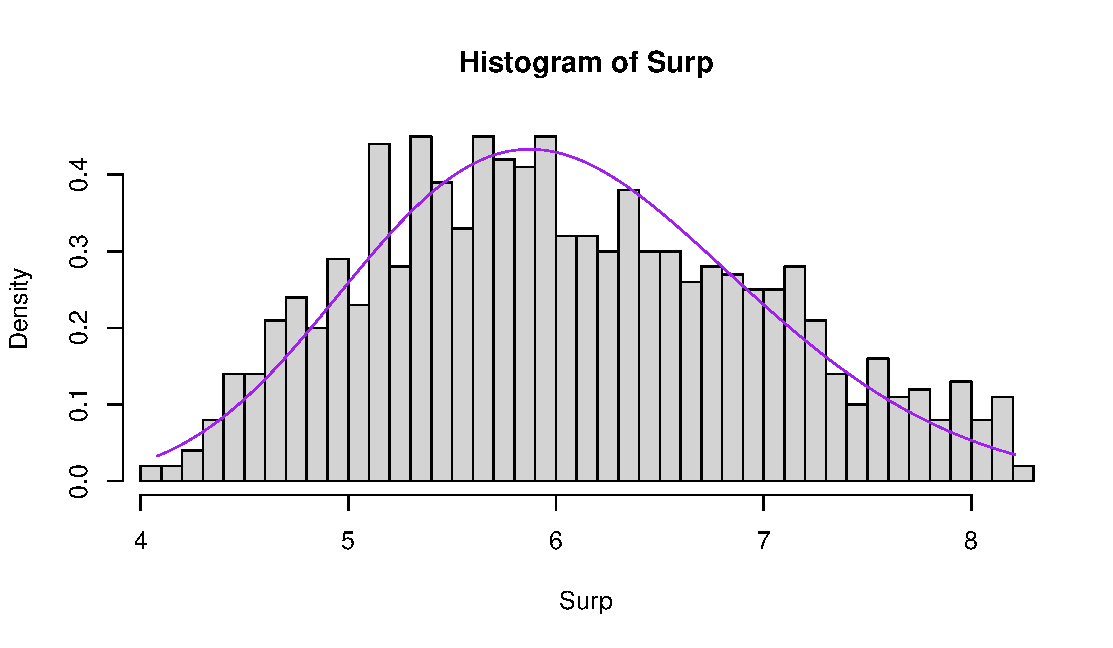
\includegraphics[trim= {0.0cm 0.00cm 0.0cm 0.0cm}, clip,  width=0.79\columnwidth]{weibull_plot.pdf}
			\caption{The estimated GEV parameters and standard errors are as follows:       location: 5.6839 (0.0314);  scale: 0.8676 (0.0229); shape: -0.20002 (0.0271).}
			\label{fig:one}
		\end{center}
		%
	\end{figure}
\end{example}

\begin{example}
	Now, let us return to the normal example, which, from our theoretical results, we know should give rise to surprisals that exhibit Gumbel like behavior. To see that this is indeed the case,  consider that we observe data generated according to
	$$
		Y_i\stackrel{iid}{\sim} \mathcal{N}(\mu=1,\sigma=1)\;(i=1,\dots,n).
	$$
	In this example, we know that the surprisal $S_i$ will have a sub-exponential tail and that $M_n=\max\{S_1,\dots,S_n\}$ should eventually resemble a GEV distribution where the shape parameter $\xi=0$. To verify this, we generate $R=1000$ independent samples of size $n=1000$ from the normal distribution with mean and variance both equal to unity, and for each $r=1,\dots,1000$ we calculate $M_n^{(r)}=\max\{S_1^{(r)},\dots,S_n^{(r)}\}$. We plot the histogram of $\{M_n^{(r)}\}_{r=1}^{1000}$ and compare this with the fitted GEV distribution in \cref{fig:two}. The estimated parameters from this experiment yield an estimated shape parameter $\hat\xi_R=0.0012$, with a standard error of 0.0209, suggesting high confidence that the actual shape parameter is either zero or very close to it, and that the distribution of $M_n$ is indeed Gumbel.

	\begin{figure}[H]%[t!]
		%\vskip -1cm %-0.1in
		\begin{center}
			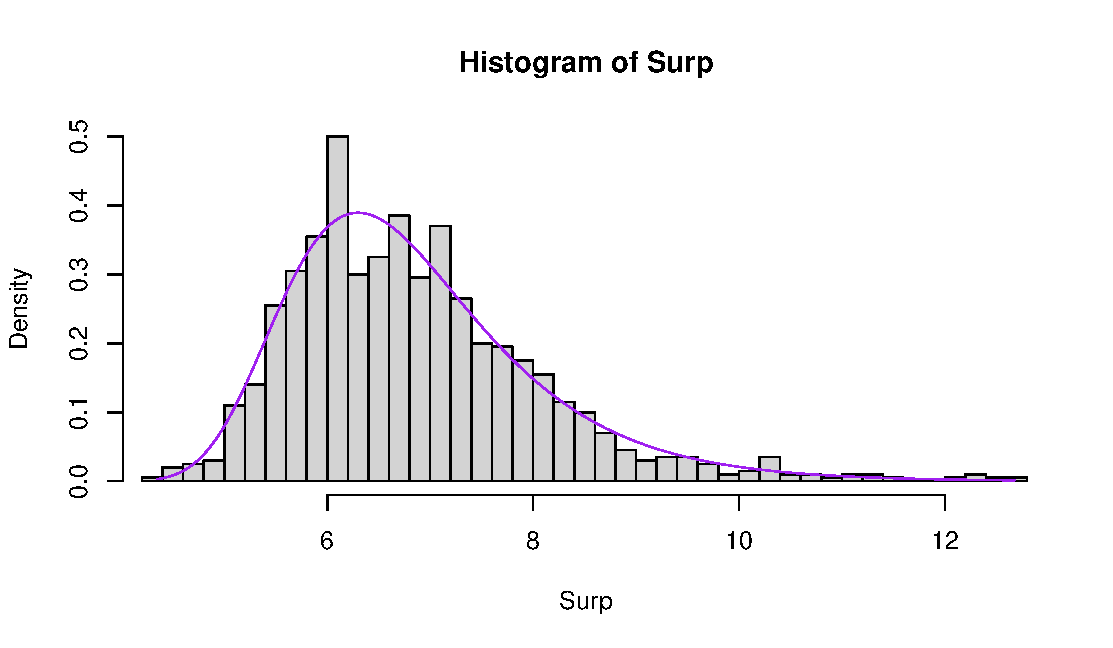
\includegraphics[trim= {0.0cm 0.00cm 0.0cm 0.0cm}, clip,  width=0.79\columnwidth]{gumbel_plot.pdf}
			\caption{The estimated GEV parameters and standard errors are given by:       location: 6.30016 (0.0332);  scale: 0.945129961 (0.0239); shape: -0.0012 (0.0209).}
			\label{fig:two}
		\end{center}

		%
	\end{figure}

\end{example}

\begin{example}
	For the last example, we consider the situation where the assumed model is Gaussian with mean and variance equal to unity, but where the observed data is actually generated from a student-t distribution with five degrees of freedom. In this case, the tails of the student-t ensure that the surprisal does not have an exponential moment, and, as discussed in \cref{thm:three_types}, the distribution of the maximum surprisal, $M_n$, will be Frechet.

	To show that this is the case we  generate $R=1000$ independent samples of size $n=1000$ from a student-t distribution with five degrees of freedom, but where the mean and variance both equal to unity, and for each $r=1,\dots,1000$ we calculate $M_n^{(r)}=\max\{S_1^{(r)},\dots,S_n^{(r)}\}$. We plot the histogram of $\{M_n^{(r)}\}_{r=1}^{1000}$ and compare this with the fitted GEV distribution in \cref{fig:three}. The estimated parameters from this experiment yield an estimated shape parameter $\hat\xi_R=0.4557$, with a standard error of 0.0294, suggesting high confidence that the actual shape parameter is positive, and that the distribution of $M_n$ is indeed Frechet.
	\begin{figure}[H]%[t!]
		%\vskip -1cm %-0.1in
		\begin{center}
			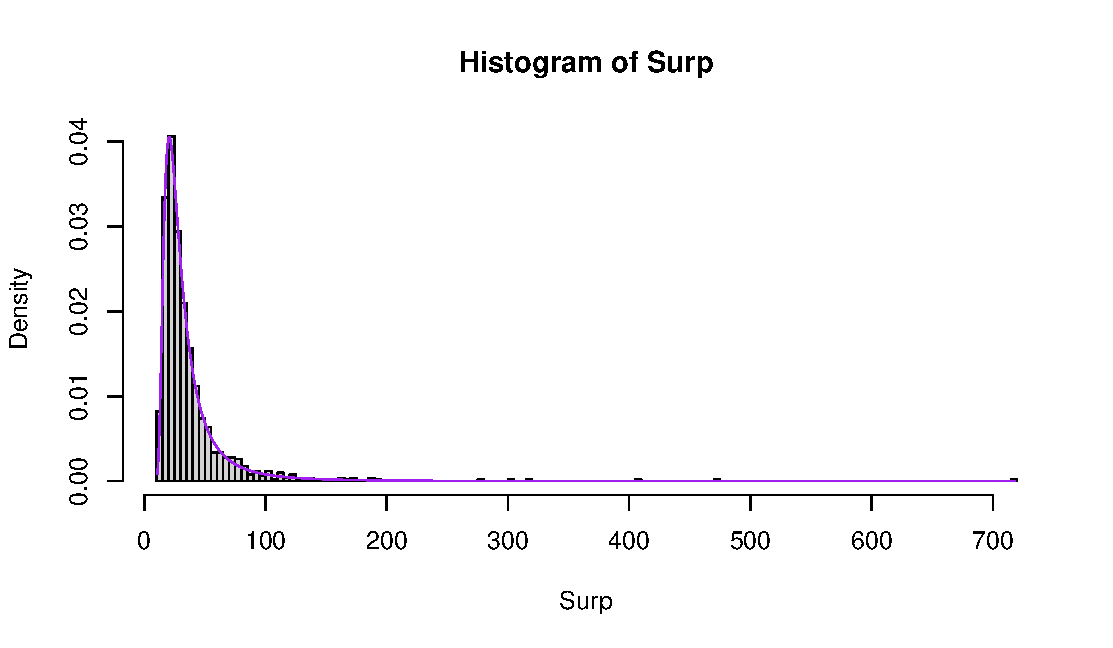
\includegraphics[trim= {0.0cm 0.00cm 0.0cm 0.0cm}, clip,  width=0.79\columnwidth]{frechet_plot.pdf}
			\caption{The estimated GEV parameters and standard errors are given by:       location: 24.0107 (0.3564);  scale: 9.9537 (0.3329); shape: 0.4557 (0.0293).}
			\label{fig:three}
		\end{center}
	\end{figure}

\end{example}

The most interesting thing from these examples from a methodological perspective is that if we get the assumed distribution of the data wrong, then this will have meaningful consequence for the behavior of the surprisal we are calculating. In particular, as the student-t example shows, when we model the data using a distribution which is assumed to have thinner tails than those of the actual data, the surprisal can have a very long/thick tail. This immediately suggests that if our goal is to check for anomalies, we should be using distributions that are somewhat robust to outliers, e.g., student-t, etc.  I've obtained similar results if you model the data with a Gaussian, but the actual data generation mechanism is exponential. In this case, the max surprisal is Frechet. However, if you had modeled the data with something like a heavy-tailed student-t, then the max surprisal is Gumble. This suggests that the model you specify is absolutely critical to understanding behavior of the max surprisal itself.

\bibliographystyle{agsm}
\bibliography{refs}

\end{document}
